\section{Dependability}
  \label{sec:Dependability}
  In the following section I will discuss how the proposed architecture for the new ACME system is dependable. In his book \textit{Software Engineering}, Ian 
  Sommerville describes the term dependability to mean \textit{'The dependability of a computer system is a property of the system that reflects its 
  trustworthiness.'} [32]. He the breaks this down into 5 sections which I will now discuss.

  \begin{figure}[H]
    \centering
    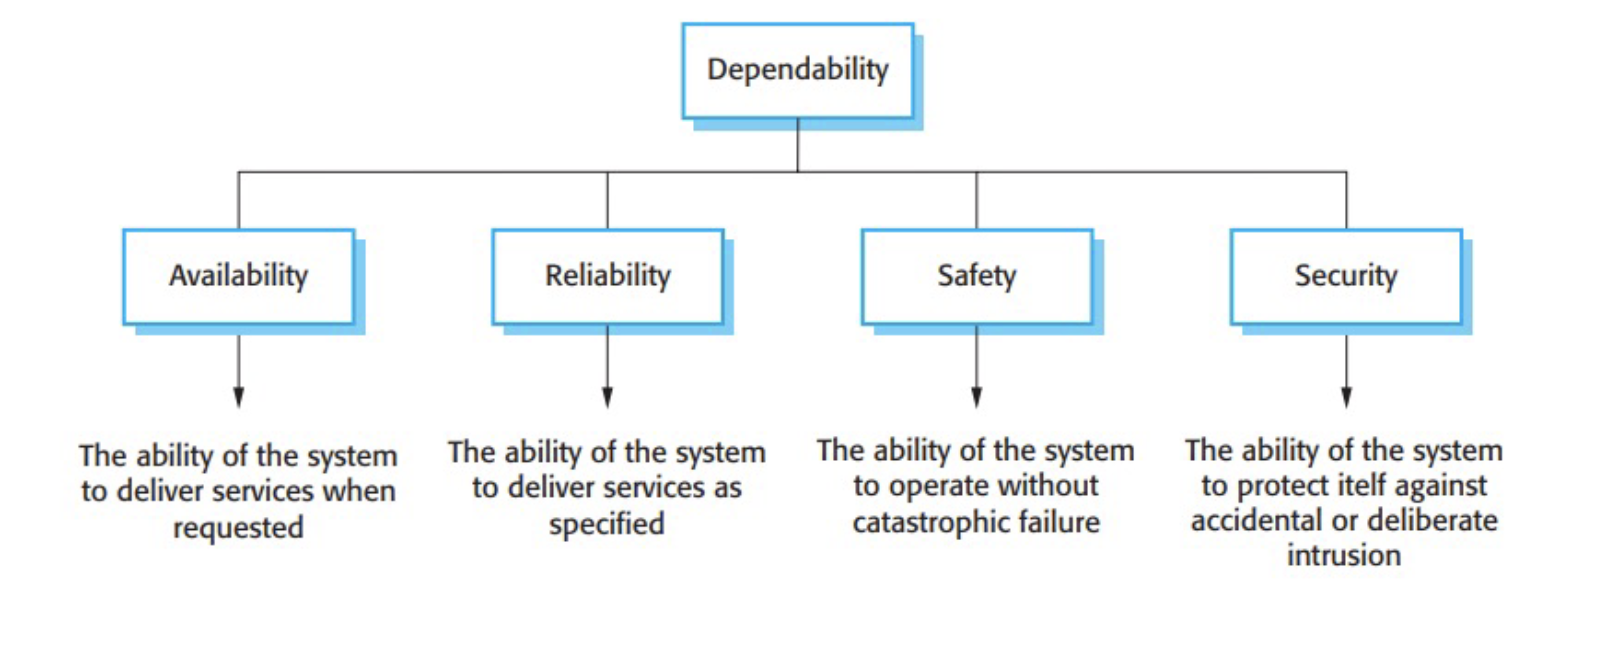
\includegraphics[width=12cm]{assets/dependability.png}
    \caption{Diagram showing the different parts of dependability [32].}
    \label{fig:dependability}
  \end{figure}

  \subsection{Reliability}
  Availability and reliability are closely linked. The image below describes the difference.
  \begin{figure}[H]
    \centering
    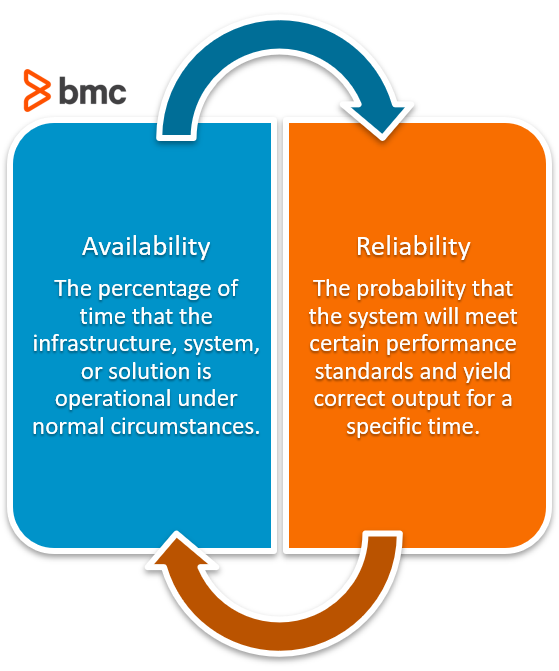
\includegraphics[width=5cm]{assets/avail-reliab.png}
    \caption{Diagram showing the difference between availability and reliability [33].}
    \label{fig:availabilityVsReliability}
  \end{figure}

  \subsubsection{Metric for ACME system reliability}

  Looking at the system designed the main component is the customer web app. This needs to successfully service as many customers as is possible.
  I have chosen the metric \textbf{POFOD = 0.0001} meaning that it is acceptable for the service to be unavailable once every 1000 requests. As this is a 
  cloud-native approach ACME has no control over what AWS will do. They themselves will have systems in place to counteract this however for 99.9\% of
  requests to succeed is still high availability.

  In order to measure this requirement AWS can help us once again. AWS provides metrics for it's components. For the web app we can check the status code
  metric, if the user receives a 2** then its OK, a 4** would be a user error and a 5** would be a server error, or downtime in this case. We can 
  then use this data to check the amount of requests that have failed due to internal server errors and check it against the metric.

  \subsection{Fault tolerance}
  Other than third party issues there are security problems that could arise. The first thing to tackle is the code itself, the code should be written in 
  a memory safe language. Non-memory safe languages (such as C) allow programmers direct access to memory which can result in attacks such as buffer
  overflows and use-after-free attacks [34]. Such attacks can end in system failure and sometimes allow a hacker to infiltrate the system. For this 
  reason I would suggest ACME use a language like Python. Not only is it memory safe, but it's got a vibrant community and an older study showed
  that the total code written and time spent writing was the lowest out of a handful of other languages [35].

  Ian Sommerville outlines 8 steps for dependable programming guidelines [32]. I will now go through each one and give examples of how ACMEs' system can 
  handle issues in that area.

  \begin{enumerate}
    \label{sec:PoLP}
    \item \textit{Limit the visibility of information in a programme} - This can be linked to the Principle of Least Privilege (PoLP) idea which 
    \textit{'refers to an information security concept in which a user is given the minimum levels of access' [36]}. Users, both internal and external, 
    should only have access to what they need to access to do their jobs. 

    However this can also be extended in a cloud-native architecture so that the individual components of the system only need permission to access what 
    they need to function. For example The payment lambda does not need access to the account lambda. This not only breaks PoLP, but also the whole idea of
    microservices being self contained operations. Steps and process should be in place and enforced to both staff and code to revoke permissions that are no
    longer needed.

    \item \textit{Check all inputs for validity} - This is vital for two reasons. The first is data integrity, you may have a schema that you want users
    data to conform to. This can make querying data easier, but also save money as you won't be having to pay for extra data storage. Additional checks such 
    as size and range checks [32] should be done, and helpful error messages returned to the client so they know what to change.
    
    However the main reason is security. In the OWASP top 10 vulnerabilities list [37] \textit{'Injection'} is 3rd and covers both XSS (Cross Site Scripting) 
    and SQL injection attacks. These are nearly always exploited via uncheck/unsanitised inputs. Both client and server side checks must be made on any data
    provided by the user. 

    \item \textit{Provide a handler for all exceptions} - This is achieved by try/catch/finally statements, or the alternative in other languages. If an 
    error occurs but is not caught, then the system could fail. In addition to this catching the error also provides an opportunity for monitoring and 
    finding potential defects in the system. Below shows the code difference between a correctly handled error and not.

    \begin{figure}[H]
      \centering
      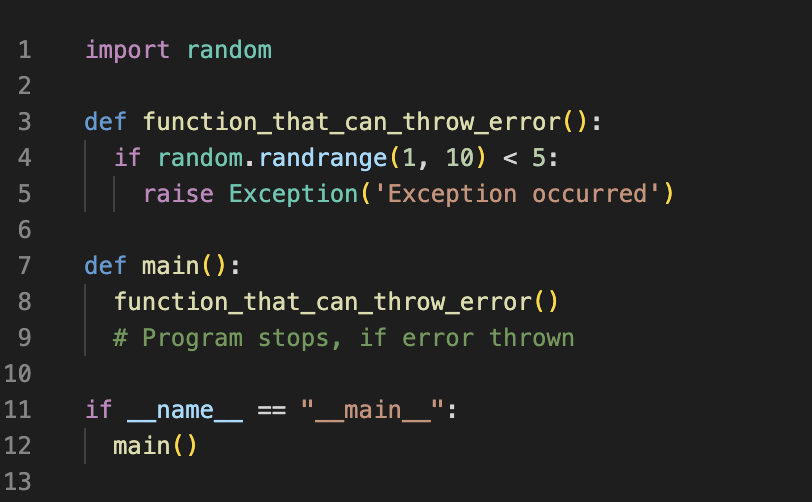
\includegraphics[width=5cm]{assets/noExceptionHandling.png}
      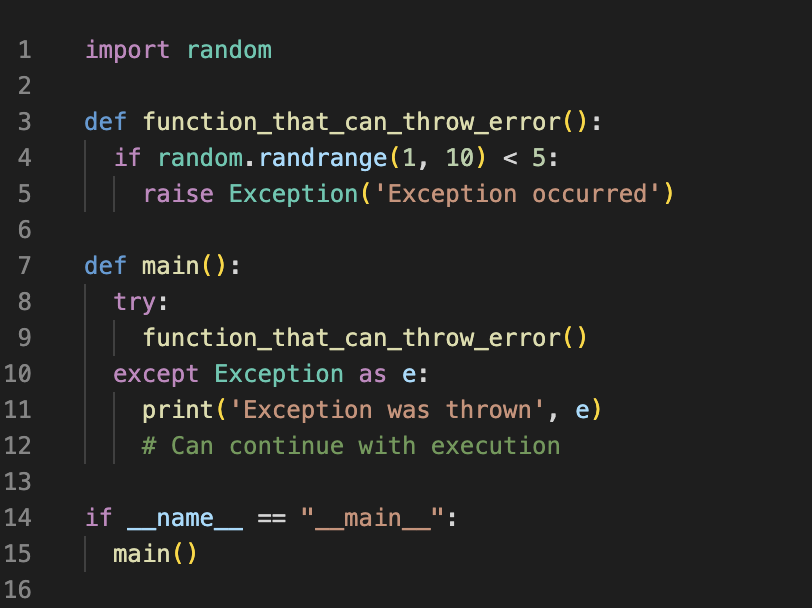
\includegraphics[width=5cm]{assets/exeptionHandling.png}
      \caption{Code demonstrating error handling (right) and no error handling (left) using Python.}
      \label{fig:errorHandling}
    \end{figure}

    \item \textit{Minimise the use of error-prone constructs} - A list of these constructs was compiled by Ian Somerville [38], however a lot of these
    are outdated, and refer to languages like C where memory allocation, array bound checking and pointers all posed issues for the developer when used
    incorrectly. However there are more modern bad coding practices that should be adhered to. One of these principles is DRY code [39], which refers to 
    clear concise code and Don't Repeat Yourself. Other issues are poor documentation. If everyone left the team then the new employees need this 
    documentation to fully understand how the system works.

    \item \textit{Provide restart capabilities} - This will be covered towards the end of this section, however making sure on system failure there
    is a procedure for critical components is vital.
    \item \textit{Check array bounds} - This is not as relevant as it would be when using an non-memory-safe language, however can still cause errors.
    There is no longer a potential memory leak, however errors can still occur when accessing out of bound ranges. Some languages like JavaScript allow
    this access and return a default value instead of erroring. However this still has to checked handlers are used to catch these errors and continue
    execution without system errors or failures occurring.

    \item \textit{Include timeouts when calling external components} - This is important as a faulty or even compromised external service could make
    your own service unavailable when trying to retrieve data from it. If one user initiated a request to the external resource that took too long 
    another user coming along in that time may not be able to access the service. In addition to this it's frustrating to the user to be sat 
    around waiting when the data may never be returned. Most libraries allow developers to add timeouts to any network request made and this is 
    implemented into the ACME system.

    \item \textit{Name all constants that represent real-world values} - This is a good practice and is sometime reffered to as \textit{'magic numbers'} [40].
    This can be troublesome when these hard-coded values are used in multiple places. Using config files for these values that can then be imported 
    throughout the project. This means if the value has to be changed, it can be changed in one place, making it much more maintainable and configurable
    in the future. It also makes code more readable instead of having seemingly random values throughout the code.

    \begin{figure}[H]
      \centering
      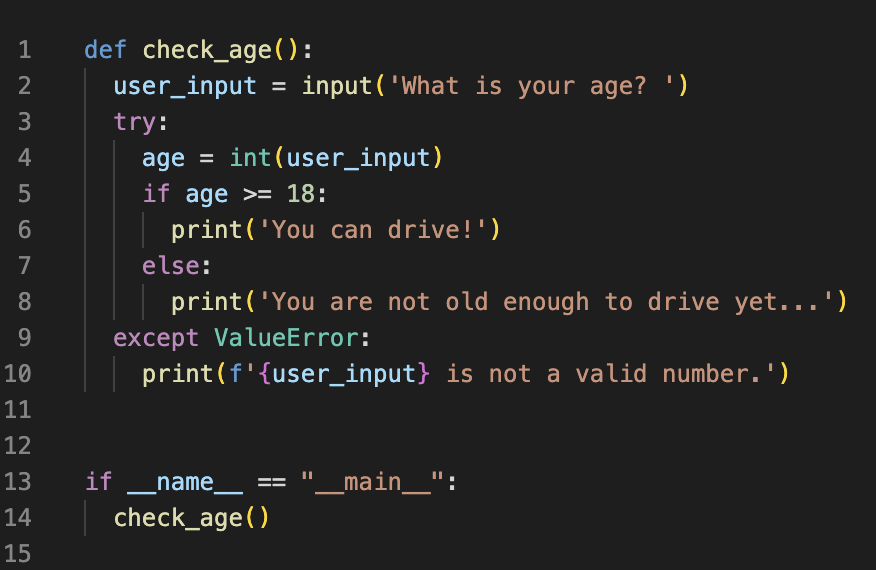
\includegraphics[width=5cm]{assets/magicNumbers.png}
      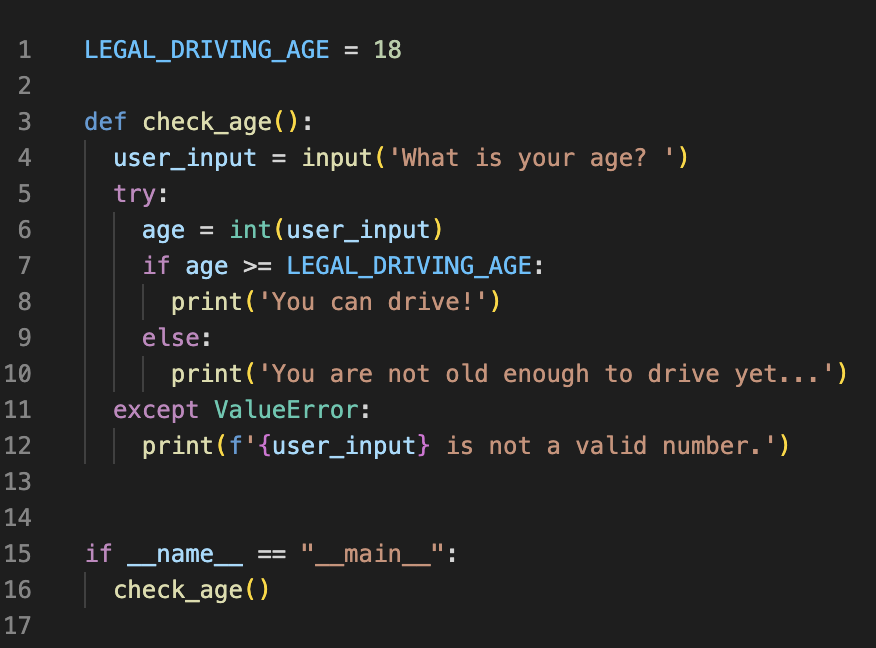
\includegraphics[width=5cm]{assets/noMagicNumbers.png}
      \caption{Code demonstrating magic numbers (left) and without (right) using Python.}
      \label{fig:magicNumbers}
    \end{figure}

  \end{enumerate}

  AWS uses metrics to track events, these can be both default and custom metrics defined in code. These metrics can then be hooked up to alarms which 
  when state changes can trigger events that are handled by the EventBridge currently in the architecture [41]. These events can then be used to trigger
  additional actions such as code rollbacks or additional checks to determine the issue.

  Rollbacks could be made possible by using Jenkins [42], which is a CI/CD provider that allows versioned deployment at the click of a button. This kind 
  of action should only be taken on components that render the service unusable though. This automation of rolling back could have other consequences to 
  other systems and therefore should be a last resort and very well tested. For example if a microservice failed, it might not be worth having this automatic
  process. However if the web front end encountered system failure it'd be worth auto restarting, especially when there is no staff currently working to 
  investigate the problems themselves.
  
  \begin{figure}[H]
    \centering
    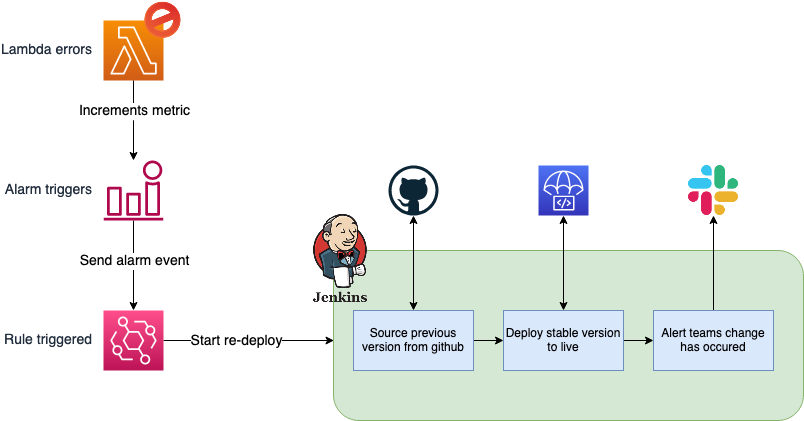
\includegraphics[width=10cm]{assets/rollbackPipeline.drawio.png}
    \caption{Diagram showing how the CI/CD pipeline of a rollback system would operate.}
    \label{fig:rollbackPipeline}
  \end{figure}
  
  \subsection{Difference between safety and security threats}

  Safety and security are not the same things when it comes to software, a definition for safety is a:
  \begin{quote}
    \textit{'should never damage people or environment even though the system fails'} [43]
  \end{quote}

  Where as security can described as:
  \begin{quote}
    \textit{'a system attribute that reflects the ability of the system to protect itself from external attacks, which may be accidental or deliberate.'} [43]
  \end{quote}

  Despite this there are situations in which these two can cross over fully. A german hospital was hacked and a woman ended up dying due the hack forcing her 
  to be transported to another hospital. This was deemed \textit{'the first known case of a life being lost as a result of a hack'} [44].
  In the rest of this section I will discuss how ACMEs' system protects/avoids the two above issues.

  \subsection{Safety}
  Safety of a system can often times be linked to harming other peoples health. The system ACME has created can't directly do that, however could have 
  indirect consequences. One issue is financial, a bug in the system could do severe harm to someone financially. There is also a chance cars provided 
  are faulty or the person driving them has provided fake ID in order to gain access to the vehicle, then going and causing people harm by not knowing 
  how to drive correctly.

  Lets starts by discussing financial issues, I previously talked about debouncing being a way to stop users accidentally performing an action more than
  once. But there are other ways to stop this financial damage. Simple things like making sure a user has to confirm there purchase after the initial 
  action can stop accidental purchases. However issues may occur despite these safeguards, because of this ACME offers a support email that is regularly
  monitored to help customers who have problems. This will hopefully stop any harm coming to customers as their funds should be returned promptly.

  To verify drivers are who they say they are ACME has multiple checks keys are given to a customer. The UK government offers a service to check 
  the validity of individuals driving licenses [45], which will be used when the customer creates an account to rent a vehicle with. However to 
  add further security to this, drivers licenses must be checked when the customer comes into the lot to pick the car up. If something isn't correct,
  the customer is refunded and the car is not rented to them.

  Doing the above will help with safety concerns that could arise from ACME's system. There is always a chance something will happen that is out of 
  ACMEs' control, however if the correct steps are taken these occurrences can be minimised.

  \subsection{Security}
  Security is always an issue in software. I will discuss this in two categories, physical (real-world) security and software security.

  \subsubsection{Physical}
  \vspace{0.2cm}
  Some threats of physical security are reduced due to the cloud-native approach chosen. This is due to no on-prem servers being used, therefore 
  user data is not accessible via physically plugging into the server. However there are still some threats worth discussing.

  \begin{itemize}
    \item \textit{Tailgating} - This is a method where an \textit{'unauthorized person gains physical access to an off-limits location'} [46]. This can 
    lead this individual gaining access to machines or information they shouldn't have access to. Staff training is required here as well as tight security
    policies around passes. Gates should only allow one person through at a time and staff should report any suspicious behaviour.

    \item \textit{Physical access to machines} - This can be garnered by the above method or other methods of social engineering/distraction. This shouldn't
    be too hard to prevent, as long as devices like PC are locked when the user is not there. Long and strong passwords are important protection here also.
    ACME will have a password policy that makes sure that passwords are changed every 3 months as well meet certain criteria, such as length and special
    characters contained. I don't recommend a password manager despite their ease of use as this represents a single point of failure. In addition to this
    these types of services have been hacked in the not so distant future [47]. Tools like haveibeenpwned [48] can also be used to determine whether someones
    email has been in a recent security breach.
  
  \end{itemize}

  \subsubsection{Software}
  I have spoke throughout this report about software security risks that can occur if developers are not careful. In this section I want to discuss
  more about preventative measures that can be taken to avoid software issues from happening.

  \begin{itemize}
    \item \textbf{Penetration testing} - This \textit{'is a cyberattack simulation launched on your computer system'} [49] most often carried out by a
    third party. There are 3 different approaches to this, black, grey and white box [50].

    \begin{table}[H]
      \centering
      \begin{tabular}{|l|l|}
        \hline
        \textbf{Type} & \textbf{Access Granted}   \\ \hline
        Black Box     & None                      \\ \hline
        Grey Box      & Some                      \\ \hline
        White Box     & Full Access               \\ \hline
      \end{tabular}
      \caption{Table showing pen testers access using different methodologies.}
    \end{table}

    I would recommend a mixture of black and white box pen testing. Black box simulates an attacked on the outside trying to gain access to the system.
    Whilst a white box test gives the pen tester the chance to view the inner workings of the code. This could flag any potential vulnerabilities that 
    made it through the QA/testing phase. This should be done once a year, as these services can cost 
    \textit{'anywhere between £600 to over £3000 per day'} [51].

    \item \textbf{Principle of least privilege (PoLP)} - As previously \hyperref[sec:PoLP]{\textbf{menitioned}} ACME will incorporate processes for 
    both onboarding and off-boarding new staff members. No staff member should have any privileges they do not need to do their job. Although this can seem 
    to be untrusting, however with 34\% of businesses suffering attacks from insiders [52] and 66\% of companies being more worried about an internal attack 
    than a external attack [52] highlights the potential issue.

    \item \textbf{QA validation/testing} - The value of testing is discussed more in the \hyperref[sec:Testing]{\textbf{Testing}} section.
    
    \item \textbf{Code reviews} - Code reviews act as a \textit{'second opinion'} [53] on newly implemented code. Another developer should always read any 
    code that plans to be released to a live environment to help stop bugs reaching consumers.

    \item \textbf{Strict dependency selection} - ACME should use only well known and tested external dependencies. In addition to this these should be checked
    into code so other developers can review them before live release. There have been multiple instances [54] where packages have been 
    \textit{'typo-squatted'} [55] and made their way to consumers.
    
    \item \textbf{Firewalls/blacklists} - AWS offers services such as WAF [56] to help protect customers against some forms of attacks. An extra layer can be 
    added to this. Software can be written to determine malicious or concerning usage of the web app, such as excessive requests (DDos) attack [57]. 
    These can then be put onto a blacklist and their requests can be dropped from then on.
  \end{itemize}

\newpage
